\section{Super-Admin}

Di seguito vengono elencati i casi d'uso per il super-admin.

\newpage

\subsection{Casi d'Uso}

\subsection{UC-S 0}

    \begin{figure}[h]
      \begin{center}
        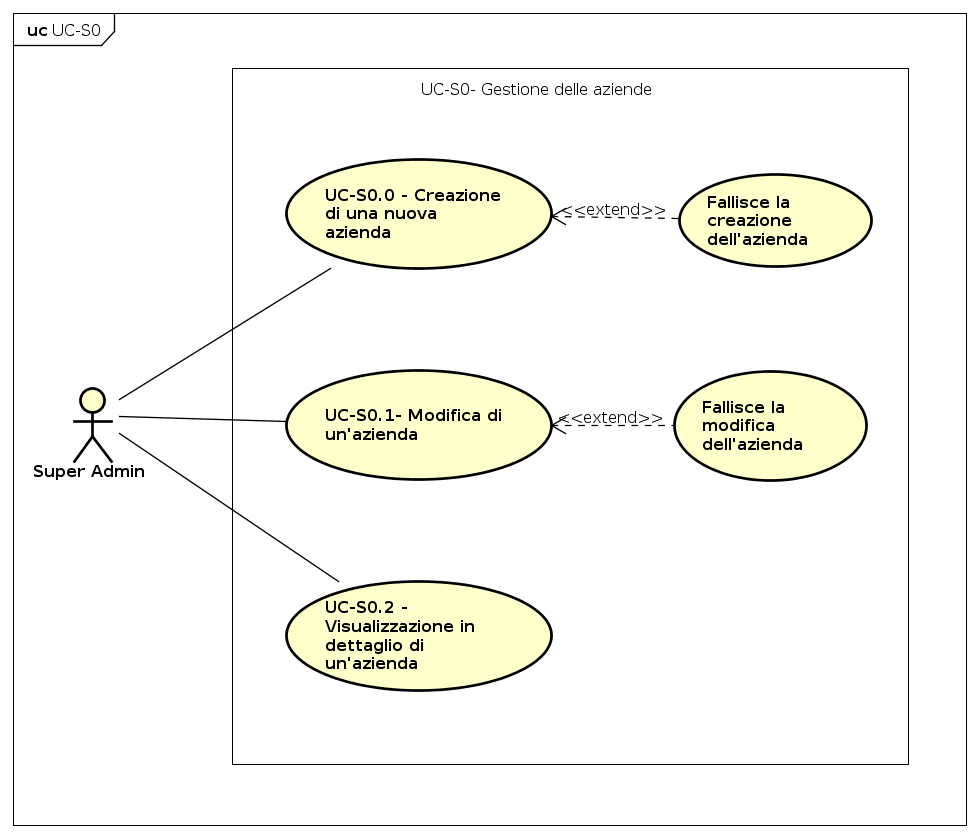
\includegraphics[width=12cm]{res/img/UCSuperadmin/UCS0.png}
      \caption{UC-S 0 - Gestione \textit{Company}}
      \end{center} 
    \end{figure}    
    
    %Tabella 
    \begin{center}
      \bgroup
      \def\arraystretch{1.8}     
      \begin{longtable}{  p{3.5cm} | p{8cm} } 
        
        \hline
        \multicolumn{2}{ | c | }{ \cellcolor[gray]{0.9} \textbf{UC-S 0 - Gestione aziende}} \\ 
        \hline
        
        \textbf{Attori Primari} & Super-Admin.\\  
        \textbf{Precondizioni}  & l'applicazione mostra al superadmin la pagina di gestione delle aziende.  \\ 
        
        \textbf{Postcondizioni} & l'applicazione mostra al superadmin la pagina di gestione delle aziende. \\ 
        \textbf{Scenario principale} & 1. il superadmin pu\`o creare una nuova \textit{Company} (UC-S 0.0). 
        
        2. il superadmin può visualizzare il dettaglio di una \textit{Company}.
        
        3. il superadmin pu\`o modificare i dati di una \textit{Company}.  \\ 
        
        \textbf{Estensioni} & 1. fallisce l'inserimento di una nuova \textit{Company}.
        
        2. fallisce la modifica dei dati di una \textit{Company}. \\
      \end{longtable}
      \egroup
    \end{center}

\subsection{UC-S 0.0}
    \begin{figure}[h]
      \begin{center}
        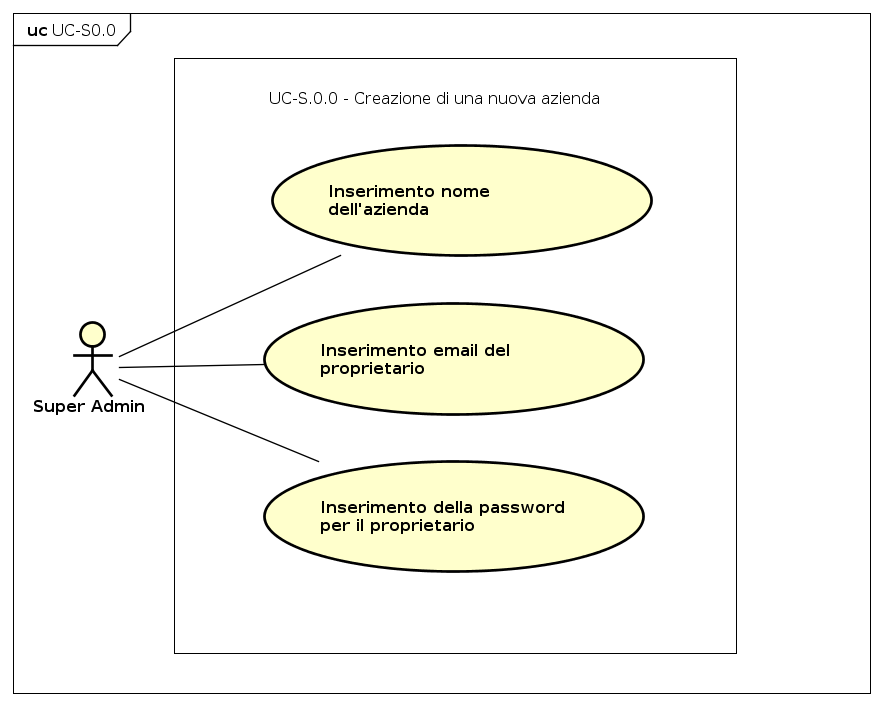
\includegraphics[width=12cm]{res/img/UCSuperadmin/UCS0.0.png}
      \caption{UC-S 0.0 - Creazione di una nuova \textit{Company}}
      \end{center} 
    \end{figure}    
    
    %Tabella 
    \begin{center}
      \bgroup
      \def\arraystretch{1.8}     
      \begin{longtable}{  p{3.5cm} | p{8cm} } 
        
        \hline
        \multicolumn{2}{ | c | }{ \cellcolor[gray]{0.9} \textbf{UC-S 0.0 - Creazione di una nuova azienda}} \\ 
        \hline
        
        \textbf{Attori Primari} & Super-Admin.\\  
        \textbf{Precondizioni}  & il sistema fornisce al super-admin un form di registrazione.  \\ 
        
        \textbf{Postcondizioni} & il sistema ha aggiunto una nuova \textit{Company} e il suo owner. \\ 
        \textbf{Scenario principale} & 1. l'attore inserisce il nome della \textit{Company}.
        
        2. l'attore inserisce la propria email.
        
        3. l'attore inserisce una password \\ 
        \textbf{Estensioni} & 1. la \textit{Company} esiste gi\`a. 
        
        2. la email inserita \`e gi\`a stata usata. \\
      \end{longtable}
      \egroup
    \end{center}

\subsection{UC-S 0.1}
    \begin{figure}[h]
      \begin{center}
        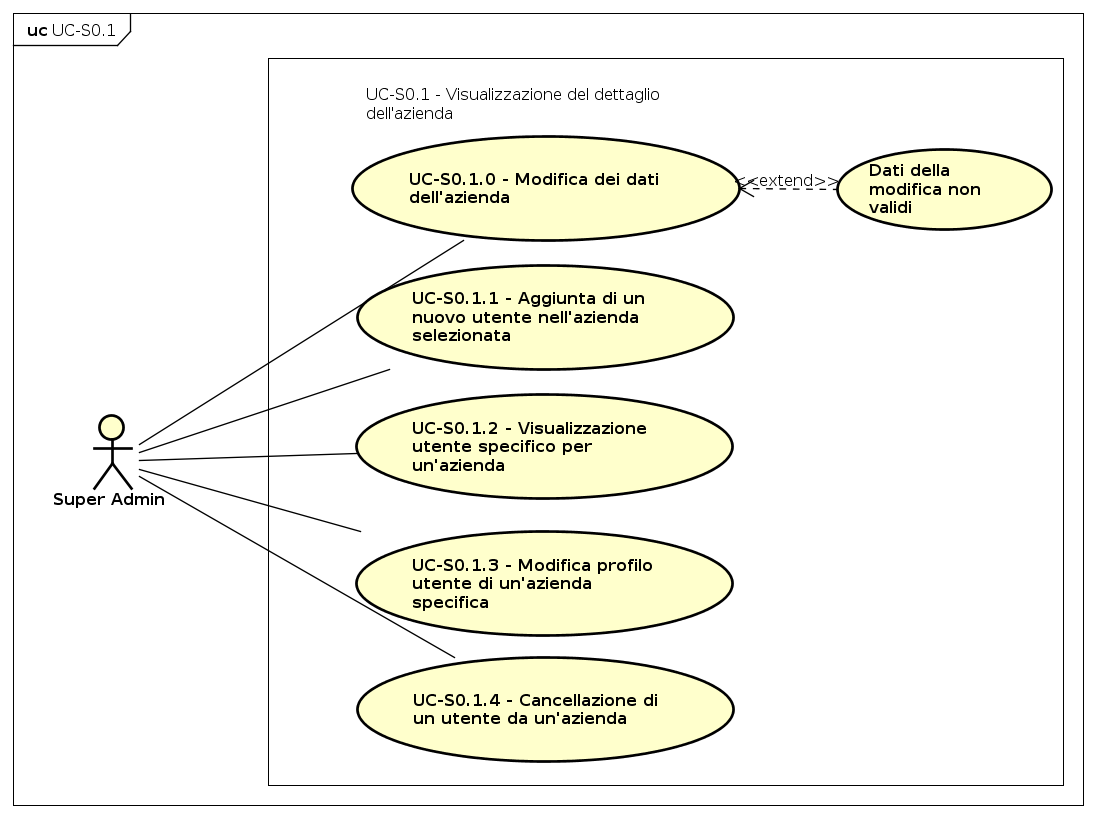
\includegraphics[width=12cm]{res/img/UCSuperadmin/UCS0.1.png}
      \caption{UC-S 0.1 - Visualizzazione dettaglio di azienda}
      \end{center} 
    \end{figure}    
    
    %Tabella 
    \begin{center}
      \bgroup
      \def\arraystretch{1.8}     
      \begin{longtable}{  p{3.5cm} | p{8cm} } 
        
        \hline
        \multicolumn{2}{ | c | }{ \cellcolor[gray]{0.9} \textbf{UC-S 0.1 - Visualizzazione dettaglio di \textit{Company}}} \\ 
        \hline
        
        \textbf{Attori Primari} & Super-Admin\\  
        \textbf{Precondizioni}  & l'applicazione mette diposizione la pagina di visualizzazione dei dettagli di una \textit{Company}.  \\ 
        
        \textbf{Postcondizioni} & l'applicazione ha reindirizzato il super-admin alla pagina di visualizzazione della \textit{Company} selezionata. \\
        
        \textbf{Scenario principale} & 1. il superadmin può modificare i dati della \textit{Company}(UC-S 0.1.0);  
        
        2. il superadmin può aggiungere un nuovo utente della \textit{Company};
        
        3. il superadmin può visualizzare uno specifico utente della \textit{Company}; 
        
        4. il super-admin pu\`o modificare i dati di uno specifico utente. \\ 
        
        \textbf{Estensioni} & 1. fallimento della modifica dei dati della \textit{Company};
        
        2. fallimento dell'aggiunta di un nuovo utente;
        
        3. fallimento modifica utente. \\
      \end{longtable}
      \egroup
    \end{center}


\subsection{UC-S 0.1.0}
    \begin{figure}[h]
      \begin{center}
        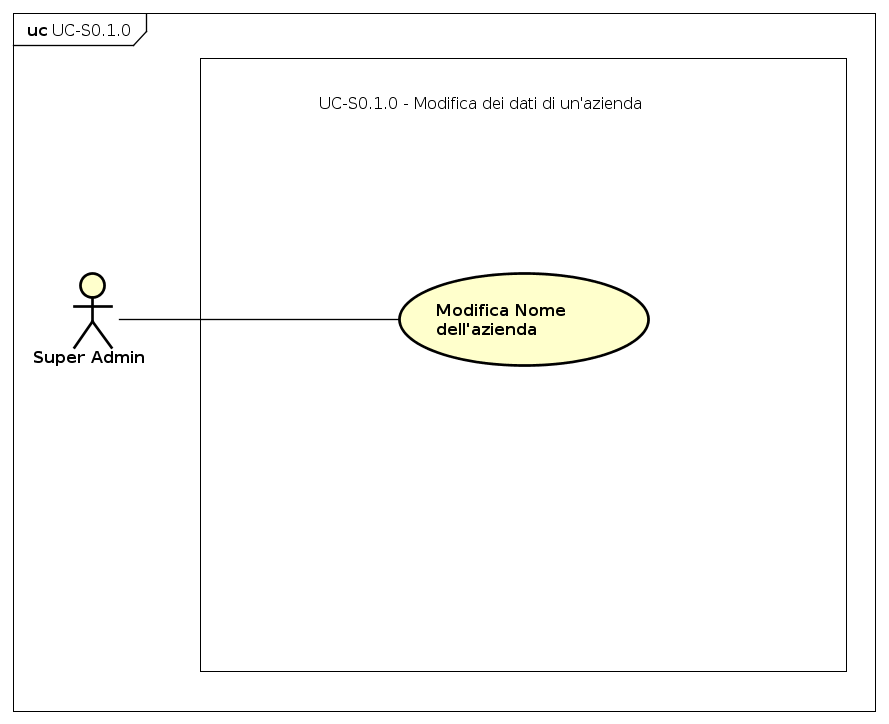
\includegraphics[width=12cm]{res/img/UCSuperadmin/UCS0.1.0.png}
      \caption{UC-S 0.1.0 - Modifica dei dati di una \textit{Company}}
      \end{center} 
    \end{figure}    
    
    %Tabella 
    \begin{center}
      \bgroup
      \def\arraystretch{1.8}     
      \begin{longtable}{  p{3.5cm} | p{8cm} } 
        
        \hline
        \multicolumn{2}{ | c | }{ \cellcolor[gray]{0.9} \textbf{UC-S 0.1.0 - Modifica dei dati di una \textit{Company}}}. \\ 
        \hline
        
        \textbf{Attori Primari} & Super-Admin.\\  
        \textbf{Precondizioni}  & l'applicazione mostra il form per la modifica dei dati della \textit{Company} selezionata.  \\ 
        
        \textbf{Postcondizioni} & il sistema ha modificato il profilo della \textit{Company} sulla base dei dati inseriti dal super-admin.  \\ 
        \textbf{Estensioni} & 1. fallimento della modifica.
      \end{longtable}
      \egroup
    \end{center}

\subsection{UC-S 0.1.1}
    \begin{figure}[h]
      \begin{center}
        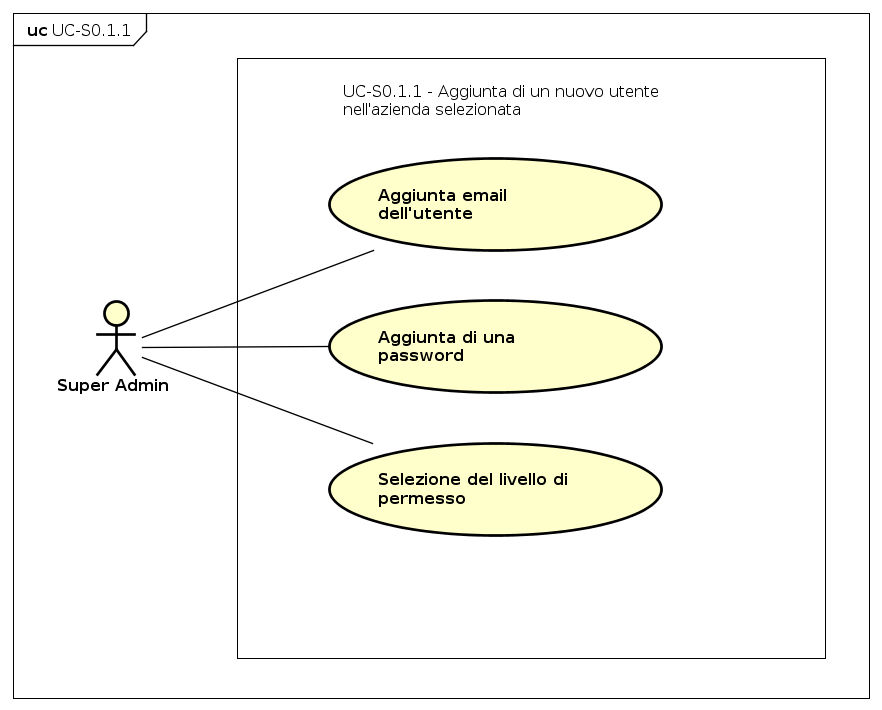
\includegraphics[width=12cm]{res/img/UCSuperadmin/UCS0.1.1.png}
      \caption{UC-S 0.1.1 - Aggiunta di un nuovo utente nella \textit{Company} selezionata}
      \end{center} 
    \end{figure}    
    
    %Tabella 
    \begin{center}
      \bgroup
      \def\arraystretch{1.8}     
      \begin{longtable}{  p{3.5cm} | p{8cm} } 
        
        \hline
        \multicolumn{2}{ | c | }{ \cellcolor[gray]{0.9} \textbf{UC-S 0.1.1 - Aggiunta di un nuovo utente nella \textit{Company} selezionata}} \\ 
        \hline
        
        \textbf{Attori Primari} & Super-Admin.\\  
        \textbf{Precondizioni}  & l'applicazione mostra il form per l'aggiunta di un nuovo utente.  \\ 
        
        \textbf{Postcondizioni} & il sistema ha aggiunto un nuovo utente associandolo alla \textit{Company} precedentemente selezionata.  \\ 
      \end{longtable}
      \egroup
    \end{center}

\subsection{UC-S 0.1.2}
    \begin{figure}[h]
      \begin{center}
        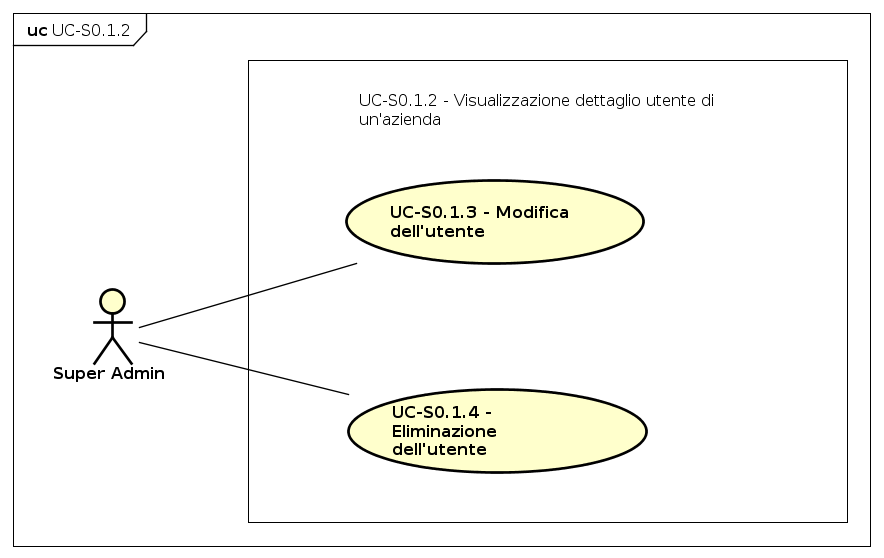
\includegraphics[width=12cm]{res/img/UCSuperadmin/UCS0.1.2.png}
      \caption{UC-S 0.1.2 - Visualizzazione in dettaglio di un utente della \textit{Company}}
      \end{center} 
    \end{figure}    
    
    %Tabella 
    \begin{center}
      \bgroup
      \def\arraystretch{1.8}     
      \begin{longtable}{  p{3.5cm} | p{8cm} } 
        
        \hline
        \multicolumn{2}{ | c | }{ \cellcolor[gray]{0.9} \textbf{UC-S 0.1.2 - Visualizzazione in dettaglio di un utente dell'azienda}} \\ 
        \hline
        
        \textbf{Attori Primari} & Super-Admin\\  
        \textbf{Scopo e descrizione} & il super-admin entra nella pagina di visualizzazione di un utente, nella quale pu\`o ispezionarne il profilo, inoltre pu\`o essere reindirizzato alle pagine di modifica ed eliminazione del utente in questione.
        \textbf{Precondizioni}  & il sistema presenta la pagina di visualizzazione in dettaglio di un utente;  \\ 
        
        \textbf{Postcondizioni} & il sistema ha ricevuto l'input dall'attore.  \\ 
         \textbf{Scenario principale} & 1. il super-admin pu\`o modificare il profilo dell'utente; 
         
         2. il super-admin pu\`o eliminare l'utente.  \\
        
     
     \end{longtable}
      \egroup
    \end{center}

\subsection{UC-S 0.1.3}
    \begin{figure}[h]
      \begin{center}
        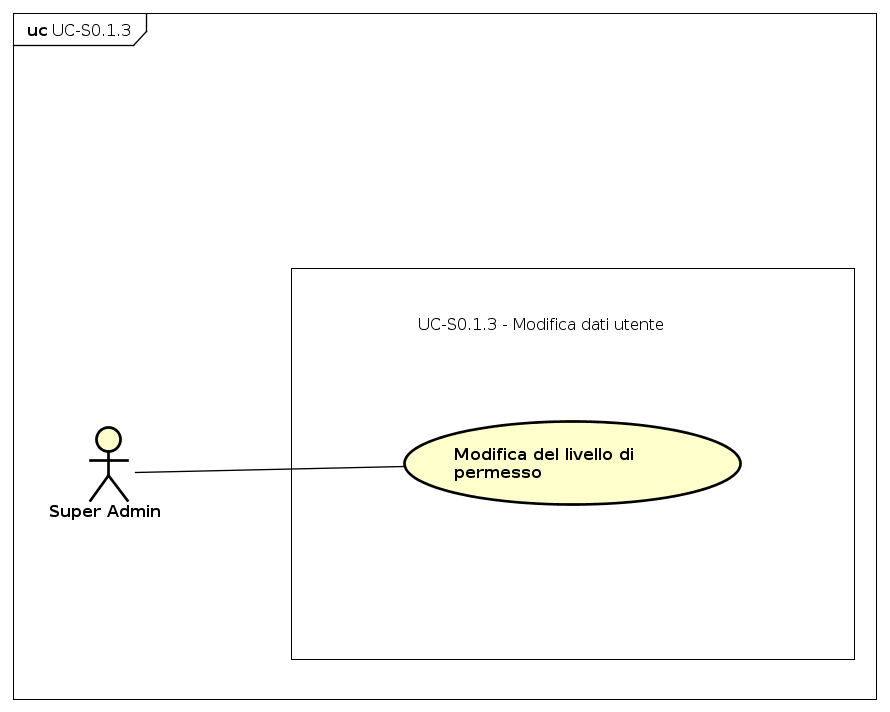
\includegraphics[width=12cm]{res/img/UCSuperadmin/UCS0.1.3.png}
      \caption{UC-S 0.1.3 - Modifica del profilo di un utente}
      \end{center} 
    \end{figure}    
    
    %Tabella 
    \begin{center}
      \bgroup
      \def\arraystretch{1.8}     
      \begin{longtable}{  p{3.5cm} | p{8cm} } 
        
        \hline
        \multicolumn{2}{ | c | }{ \cellcolor[gray]{0.9} \textbf{UC-S 0.1.3 - Modifica del profilo di un utente }} \\ 
        \hline
        
        \textbf{Attori Primari} & Super-Admin\\  
        \textbf{Scopo e descrizione} & l'attore entra nella pagina di modifica dell'utente, nella quale ha la possibilit\`a
        di modificarne ruolo e password.
      
        \textbf{Precondizioni}  & l'applicazione predispone un form di modifica del profilo. \\ 
        
        \textbf{Postcondizioni} & il sistema ha modificato il profilo dell'utente sulla base di quanto inserito dall'attore. \\ 
         \textbf{Scenario principale} & 1. l'utente ha la possibilit\`a di modificare la tipologia dell'utente. 
        
        
         \textbf{Estensioni} & 1. uscita dalla pagina senza salvataggio delle modifiche.  \\
     
     \end{longtable}
      \egroup
    \end{center}



\subsection{UC-S 0.1.4}
    \begin{figure}[h]
      \begin{center}
        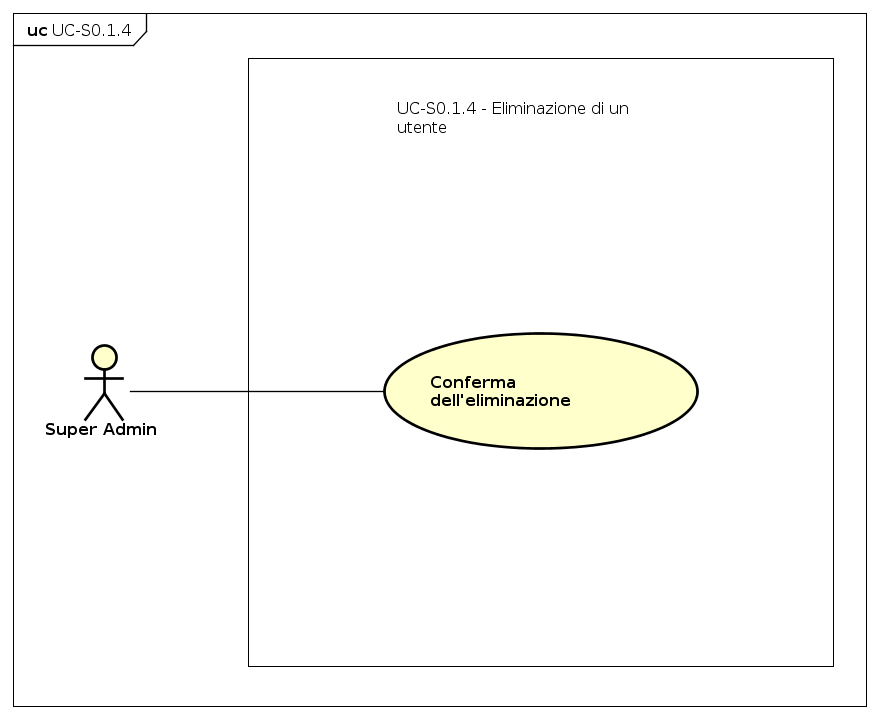
\includegraphics[width=12cm]{res/img/UCSuperadmin/UCS0.1.4.png}
      \caption{UC-S 0.1.4 - Eliminazione di un utente}
      \end{center} 
    \end{figure}    
    
    %Tabella 
    \begin{center}
      \bgroup
      \def\arraystretch{1.8}     
      \begin{longtable}{  p{3.5cm} | p{8cm} } 
        
        \hline
        \multicolumn{2}{ | c | }{ \cellcolor[gray]{0.9} \textbf{UC-S 0.1.4 - Eliminazione di un utente }} \\ 
        \hline
        
        \textbf{Attori Primari} & Super-Admin\\  
        \textbf{Scopo e descrizione} & l'attore entra nella pagina di eliminazione dell'utente, nella quale ha la possibilit\`a
        di eliminarlo.
      
        \textbf{Precondizioni}  & l'applicazione richiede la conferma dell'eliminazione dell'utente. \\ 
        
        \textbf{Postcondizioni} & il sistema ha seguito le indicazioni dell'attore. \\ 
         \textbf{Scenario principale} & 1. l'attore ha la possibilit\`a di confermare l'eliminazione; 
         
         2. l'attore ha la possibilit\`a ritirare la richiesta di eliminazione. \\
        
         \textbf{Estensioni} & 1. uscita dalla pagina senza salvataggio delle modifiche.  \\
     
     \end{longtable}
      \egroup
    \end{center}


\subsection{UC-S 1}
    \begin{figure}[h]
      \begin{center}
        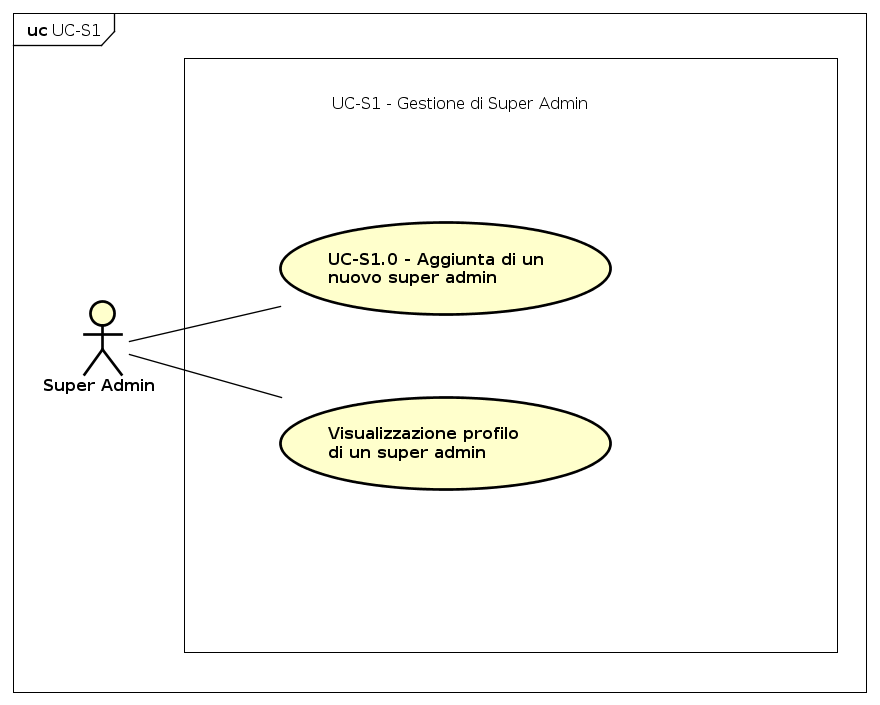
\includegraphics[width=12cm]{res/img/UCSuperadmin/UCS1.png}
      \caption{UC-S 1 - Gestione di altri super-admin}
      \end{center} 
    \end{figure}    
    
    %Tabella 
    \begin{center}
      \bgroup
      \def\arraystretch{1.8}     
      \begin{longtable}{  p{3.5cm} | p{8cm} } 
        
        \hline
        \multicolumn{2}{ | c | }{ \cellcolor[gray]{0.9} \textbf{UC-S 1 - Gestione di altri super-admin }} \\ 
        \hline
        
        \textbf{Attori Primari} & Super-Admin.\\  
        \textbf{Scopo e descrizione} & L'utente è entrato nella pagina di gestione dei super-admin. In questa pagina può aggiungere un nuovo super-admin,
vedere in un elenco quelli già presenti e poterne vedere le informazioni in dettaglio cliccando nella voce dell'elenco.
      
        \textbf{Precondizioni}  & il super-admin entra nella pagina di gestione dei super-admin.\\ 
        
        \textbf{Postcondizioni} & il sistema ha preso in carico le indicazioni dell'attore. \\ 
         \textbf{Scenario principale} & 1. l'attore ha la possibilit\`a di aggiungere un nuovo super-admin  
         
         2. l'attore ha la possibilit\`a di visualizzare in dettaglio il profilo di un super-admin esistente. \\
        
         \textbf{Estensioni} & 1. fallimento dell'inserimento di un super-admin.  \\
     
     \end{longtable}
      \egroup
    \end{center}


\subsection{UC-S 1.0}
    \begin{figure}[h]
      \begin{center}
        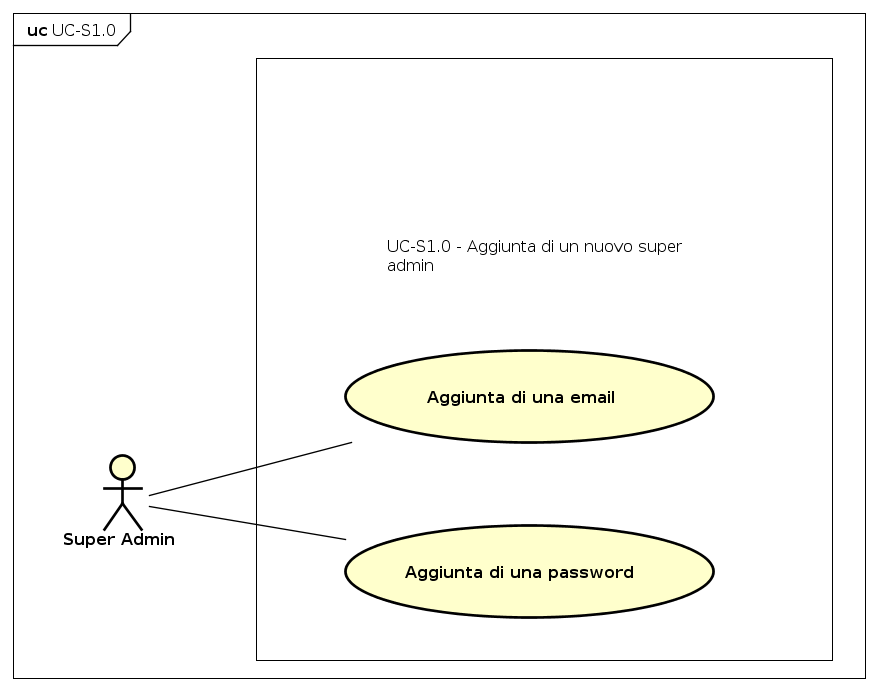
\includegraphics[width=12cm]{res/img/UCSuperadmin/UCS1.0.png}
      \caption{UC-S 1.0 - Creazione di un super-admin}
      \end{center} 
    \end{figure}    
    
    %Tabella 
    \begin{center}
      \bgroup
      \def\arraystretch{1.8}     
      \begin{longtable}{  p{3.5cm} | p{8cm} } 
        
        \hline
        \multicolumn{2}{ | c | }{ \cellcolor[gray]{0.9} \textbf{UC-S 1.0 - Creazione di un super-admin }} \\ 
        \hline
        
        \textbf{Attori Primari} & Super-Admin.\\  
        \textbf{Scopo e descrizione} & l'attore entra nella pagina di creazione di un altro super-admin. 
        Qui deve aggiungere le informazioni (email, password) necessarie per la registrazione di un nuovo super-admin.
      
        \textbf{Precondizioni}  &  l'attore entra nella pagina di creazione di un nuovo super-admin 
        \textbf{Postcondizioni} & il sistema ha creato un nuovo super-admin nel database \\ 
         \textbf{Scenario principale} & 1. l'attore inserisce l'email dell'utente da registrare; 
         
         2. l'attore aggiunge una password nell'apposito campo.\\
        
         \textbf{Estensioni} & 1. l'attore esce dalla pagina;  
         
         2. l'email inserita \`e gi\`a presente nel database e il nuovo super-admin non pu\`o essere creato.\\ 
     
     \end{longtable}
      \egroup
    \end{center}


    





